\begin{figure}[ht!]
    \centering
    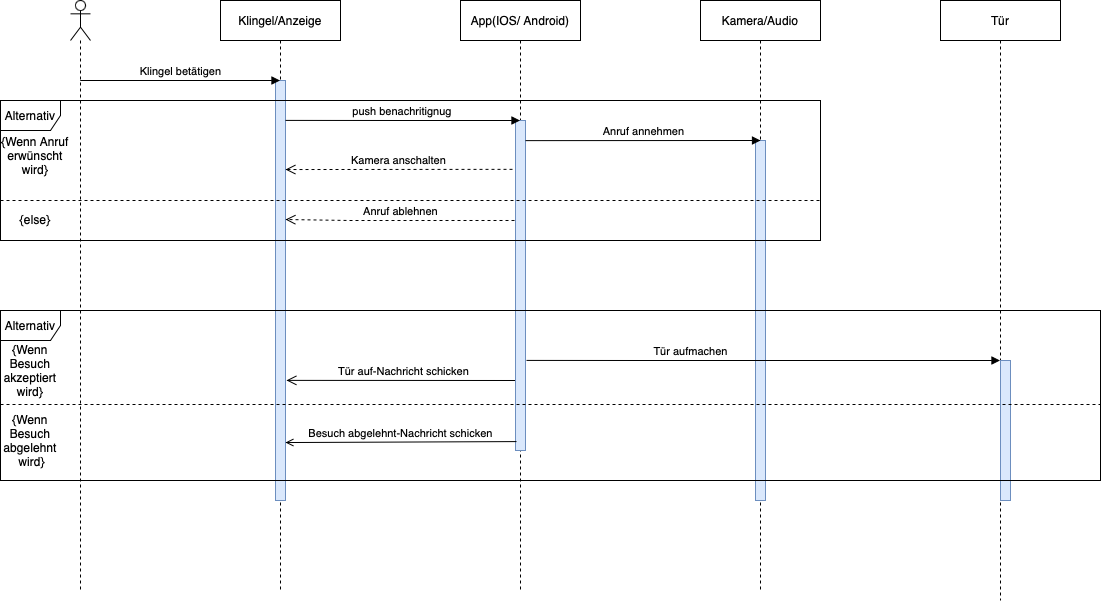
\includegraphics[width=\paperwidth-2in]{../assets/img/Klingeln bei Mehrfamilienhaus(Sequenzdiagram).drawio}
    \caption{Klingeln bei einem Mehrfamilienhaus Sequenzdiagram}
    \label{fig:klingeln-bei-einem-mehrfamilienhaus-sequenz-diagram}
\end{figure}
Beim Klingeln wird, wie in Abbildung~\ref{fig:klingeln-bei-einem-mehrfamilienhaus-sequenz-diagram} dargestellt ist, eine Push--Nachricht an die Android-- / iOS--App des Hausbesitzers gesendet.
Entscheidet er sich, den Anruf anzunehmen, werden Video und Audio über eine Annahmetaste in der App gestartet und der Video-- und Audioplayer wird gestartet.
Entscheidet er sich, den Anruf abzulehnen, sendet die App eine Ablehnungsnachricht an die Klinge Anzeige.


Nimmt der Besitzer den Besuch an, klickt er auf einen Button in der App und die App sendet eine Nachricht an die Türsteurung, um die Tür zu öffnen.
Andernfalls wird eine Nachricht an die Klinge Anzeige gesendet, dass der Besuch verweigert wird.